\documentclass[12pt]{article}
\usepackage[utf8]{inputenc}
\usepackage[english]{babel}
\usepackage{amsmath}
\usepackage{natbib}
\usepackage{graphicx}
\usepackage{hyperref}
\usepackage{caption}
\usepackage{caption,float}
\usepackage[vmargin=3cm,hmargin=3cm]{geometry}

\begin{document}

{\centering

\rule{\textwidth}{1.6pt}\vspace*{-\baselineskip}\vspace*{2pt} 
\rule{\textwidth}{0.4pt}\\[\baselineskip] 
{\LARGE Growing Degree Day}
\rule{\textwidth}{0.4pt}\vspace*{-\baselineskip}\vspace{3.2pt}
\rule{\textwidth}{1.6pt}\\[\baselineskip] 

\vspace{20mm} %5mm vertical space
\scshape % Small caps
CMSC 6950 - Computer Based Research Tools and Applications \\ [\baselineskip]
Term Project \\[\baselineskip] 
16th June, 2016 \\[\baselineskip] 
\vspace{20mm} %5mm vertical space
Submitted by \\[\baselineskip]
{\Large Xiao Wang\\Chen Wei \\Thanjida Akhter \\ Md Kamrul Hasan \\ Huizhong Liu \\ Yuan Zhi\\Maulik Rawal \par}
\vfill
{\itshape Memorial University of Newfoundland \\ St. John's, Canada.\par} 
}

\newpage

{\centering
  \section*{Abstract}
}

We selected the following cities: St.John's, Halifax, Toronto and Vancouver to complete the task in the project. Firstly, we created a auto-download python program to download the historical climate data from web. Moreover, we created a python data to calculate the accumulated GDDs and plot them for the selected cities. We also plot the accumulated GDD for several years in a selected city and for several cities in the same year. The plot for different base temperature was also included in out project. \\






\section{ \bf Introduction}
Growing degree days (GDD) is a statistical tool to measure heat accumulation and can be used to predict plant and animal development rates such as the date that a flower will bloom, an insect will emerge from dormancy, or a crop will reach maturity \cite{1}.


In our project we selected four major cities in Canada which are St.John's, Halifax, Toronto and Vancouver. We downloaded the historical data for the selected cities between 2013 and 2016, using the formula of calculating GDD, we calculated the accumulated GDD for each cites in the selected years and plotted several graphs.

Besides the plot of accumulated GDD for several years, we also did accumulated GDD plot for different cities in the same year. From those plot we could compare accumulated GDD through years or cities. 


\section{ \bf Data Processing}
\subsection{Data Collection}
In our project, firstly, we wrote a autodownload python code to automatically download all data from web for selected cities. After downloading, we read the data using python package pandas and stored  maximum and minimum daily temperature into data files.

Secondly, we wrote a python code to calculate the GDD and accumulated GDD for the selected cities from year 2013 to 2016. In the calculation we need Moreover, we plotted the accumulated GDD for different cities and years and saved them into png files. 



\subsection{Growing Degree Day Calculation}
Growing Degree Day(GDD) are calculated by taking the integral of warmth above a base temperature. Or simply, approximately equivalent to take the average temperature and minus base temperature in the following equation:

\begin{equation}
\textrm{GDD} = \left(\frac{T_{max} + T_{min}}{2}\right) - T_{base}
\end{equation}

\noindent {$T_{max}$}, {$T_{min}$}, and {$T_{base}$} are the daily maximum, daily minimum and base temperatures, respectively. Normally the maximum and minimum daily temperatures are pre-calculated before the above equation. If the maximum or minimum daily temperature is lower than the base temperature, then we set the maximum or minimum daily temperature equal to the base temperature.

For example, if the maximum daily temperature is 20, the minimum daily temperature is 5 and the base temperature is 10, we will have the GDD in the following equation:

\begin{equation}
\textrm{GDD} =\frac{20+10}{2}- 10=5
\end{equation}


\section{Graphs and Analysis}
\subsection{ \bf St.Johns }

We analyzed the historical data in 2013 for St.John's. The maximum and minimum daily temperature as figure (\ref{1}), and the accumulated GDD as figure (\ref{1.1}). From the figure (\ref{1}), we see that the maximum daily temperature for St.John's is happened in the middle of June and its value is closed to $30^{o}$C, the minimum daily temperature is happened in January and its value is closed to $-20^{o}$C.

From figure (\ref{1.1}), we see that the value of accumulated GDD for St.John's is closed to 800, it is enough for most flower blooming (need accumulated GDD higher than 500) and core maturity (need accumulated GDD higher than 800), however, it is not enough for oats maturity which need accumulated GDD higher than 1500.




\begin{figure}[H]
\begin{center}
\includegraphics[width=5.25in]{Plot/St.Johns/day_vs_temp_2013.png}

\caption{Cycle of minimum and maximum daily temperatures for St.Johns.}
\label{1}
\end{center}





\end{figure}




\begin{figure}[H]
\centering
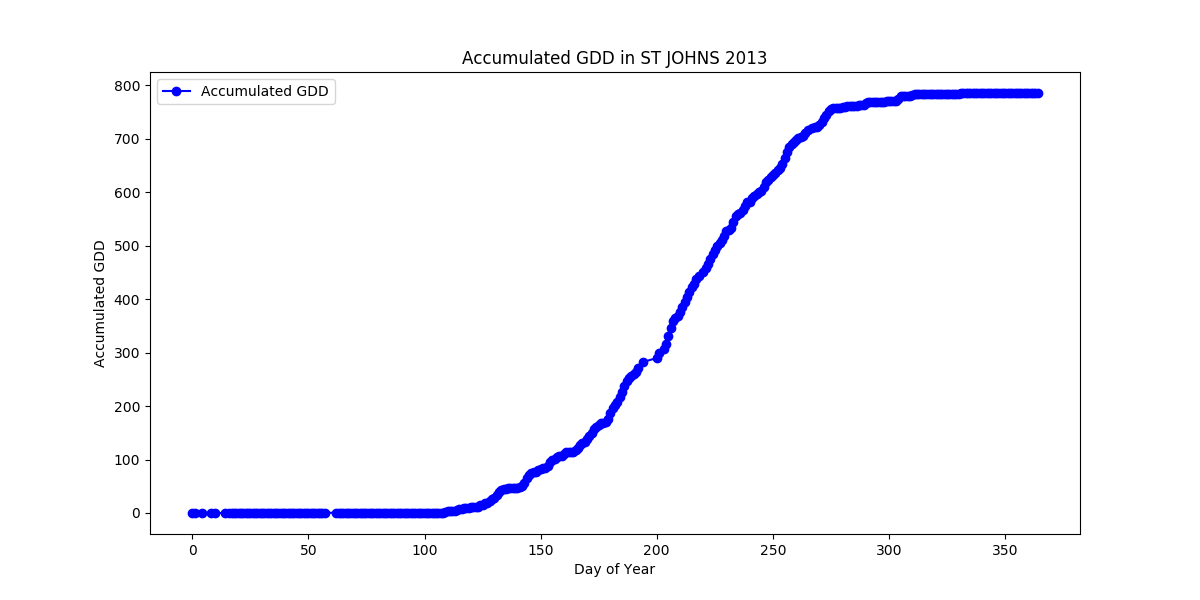
\includegraphics[width=5.25in]{Plot/stjohns.png}



\caption{Accumulated GDD for St.Johns in 2013}
\label{1.1}


\end{figure}



\subsection{ \bf Halifax }

Now we turn our attention to Halifax. From figure (\ref{2}) The maximum daily temperature of Halifax is happened to be in the end of June and its value is slightly higher than $30^{o}$C which is higher than the maximum daily temperature of St.John's. However, the minimum daily temperature is happened in the middle of February and its value is lower than $-20^{o}$C which is lower than the minimum temperature of St.John's.

From figure (\ref{2.2}), we see the value of accumulated GDD is higher than 1000 which is much higher than the value of St.John's.




\begin{center}
\begin{figure}[H]
\includegraphics[width=5.25in]{Plot/HALIFAX/day_vs_temp_2013.png}



\caption{Cycle of minimum and maximum daily temperatures for Halifax}
\label{2}
\end{figure}
\end{center}


\begin{figure}[H]
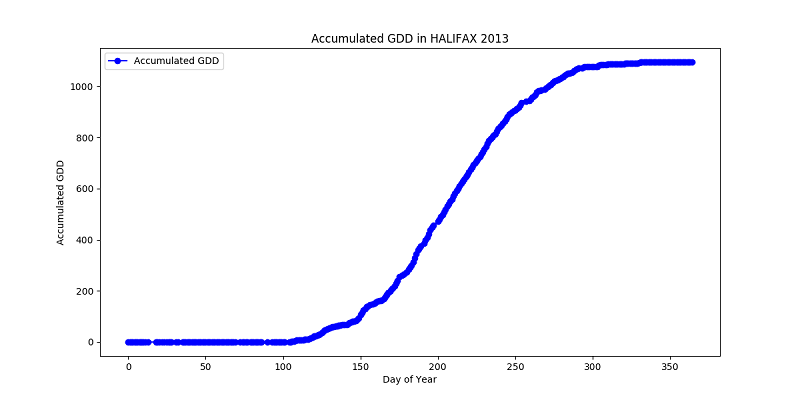
\includegraphics[width=5.25in]{Plot/halifax.png}



\caption{Accumulated GDD for Halifax in 2013}
\label{2.2}
\end{figure}






\subsection{ \bf Toronto }



From figure (\ref{3}), we can identify the value of maximum daily temperature is around $35^{o}$C, and the value of minimum daily temperature is closed to $-20^{o}$C. Toronto has a relatively hot summer compare to St.John's and Halifax. 

From figure (\ref{3.3}), the value of accumulated GDD is closed to 1400 which is much higher than St.John's as well as Halifax.

\begin{center}
\begin{figure}[H]
\includegraphics[width=5.25in]{Plot/Toronto/day_vs_temp_2013.png}



\caption{Cycle of minimum and maximum daily temperatures for Toronto.}
\label{3}
\end{figure}
\end{center}

\begin{figure}[H]
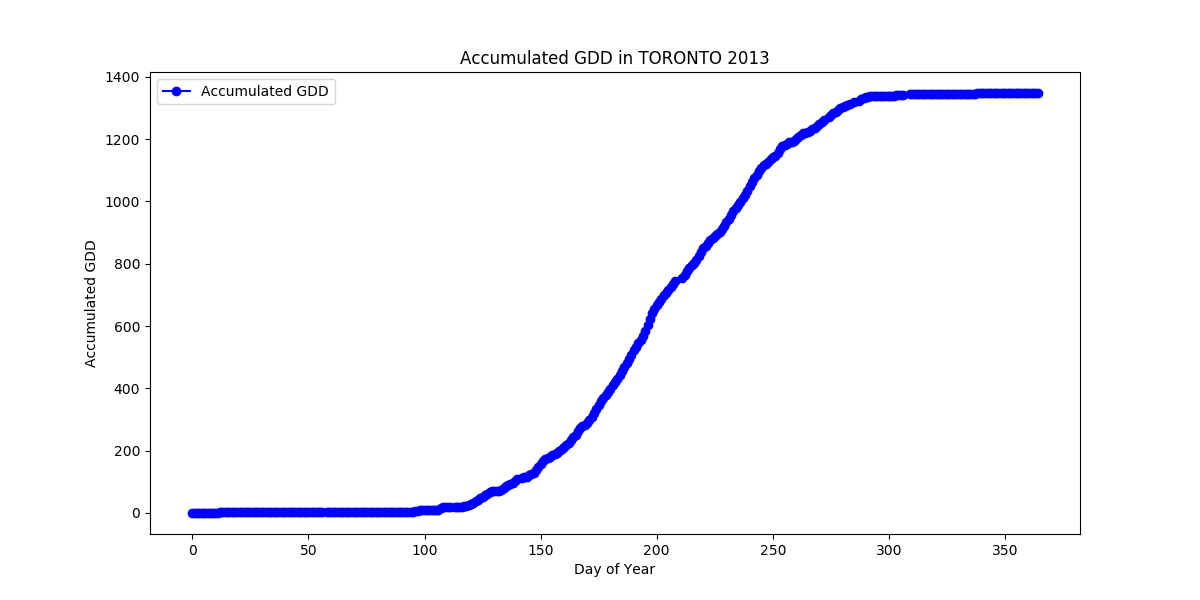
\includegraphics[width=5.25in]{Plot/toronto.png}



\caption{Accumulated GDD for Toronto in 2013}
\label{3.3}
\end{figure}





\subsection{ \bf Vancouver }
Now let us take a look at our last selected city Vancouver. From figure (\ref{4}), we see the value of maximum daily temperature is around $25^{o}$C and it happened in the end of August, however, the value of maximum daily temperature are very close through the whole summer. The minimum daily temperature is happened in the middle of December and its value is around $-5^{o}$C. Therefore, Vancouver has a mild summer and winter.


From figure (\ref{4.4}), the value of accumulated GDD is closed to 1200, which is higher than the value of St.John's and Halifax, but lower than the value of Toronto.

\begin{center}
\begin{figure}[H]
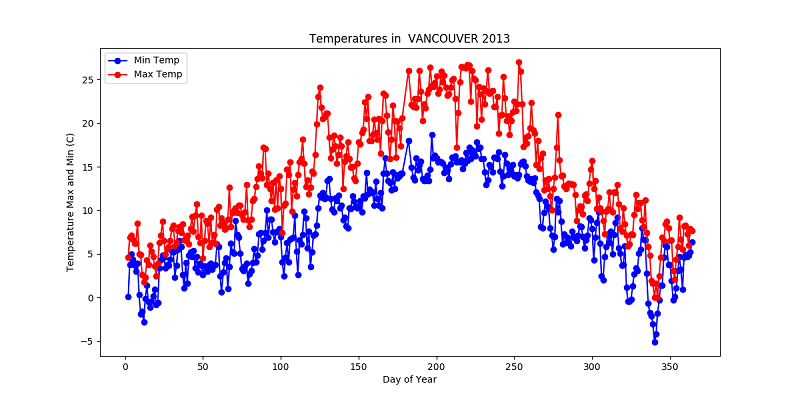
\includegraphics[width=5.25in]{Plot/VANCOUVER/day_vs_temp_2013.png}




\caption{Cycle of minimum and maximum daily temperatures for Vancouver.}
\label{4}
\end{figure}
\end{center}

\begin{figure}[H]
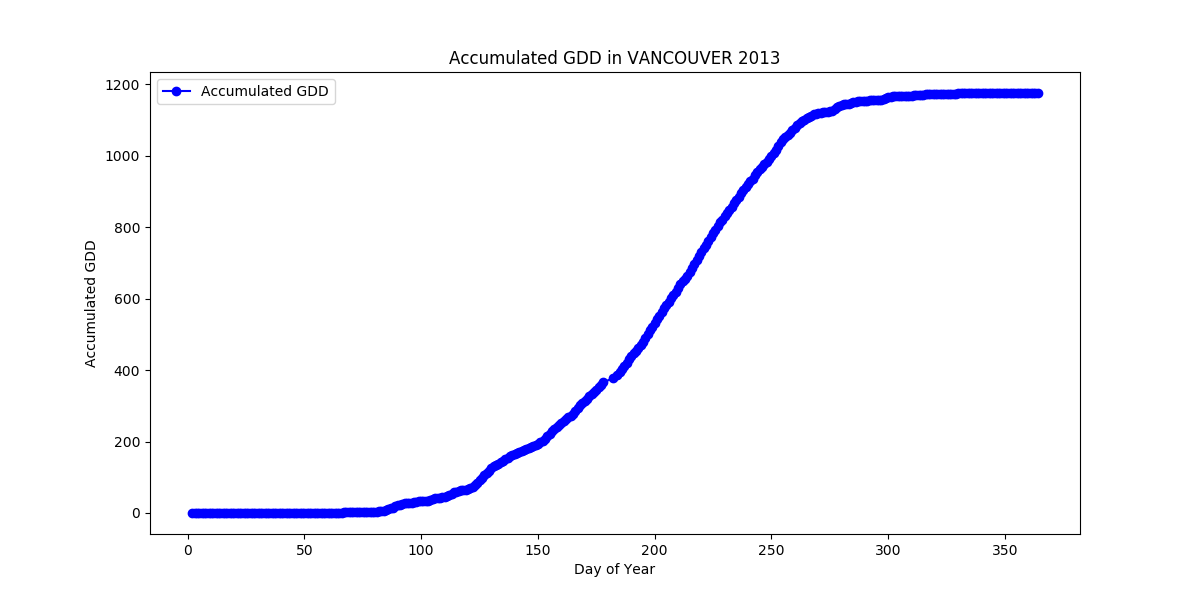
\includegraphics[width=5.25in]{Plot/vancuver.png}



\caption{Accumulated GDD for Vancouver in 2013}
\label{4.4}
\end{figure}



\subsection{ \bf Accumulated GDD in Same Year  }


\subsection{Year 2013}

In year 2013, the accumulated GDD of Toronto takes the lead, followed by Vancouver, Halifax and St.John's.
\begin{figure}[H]
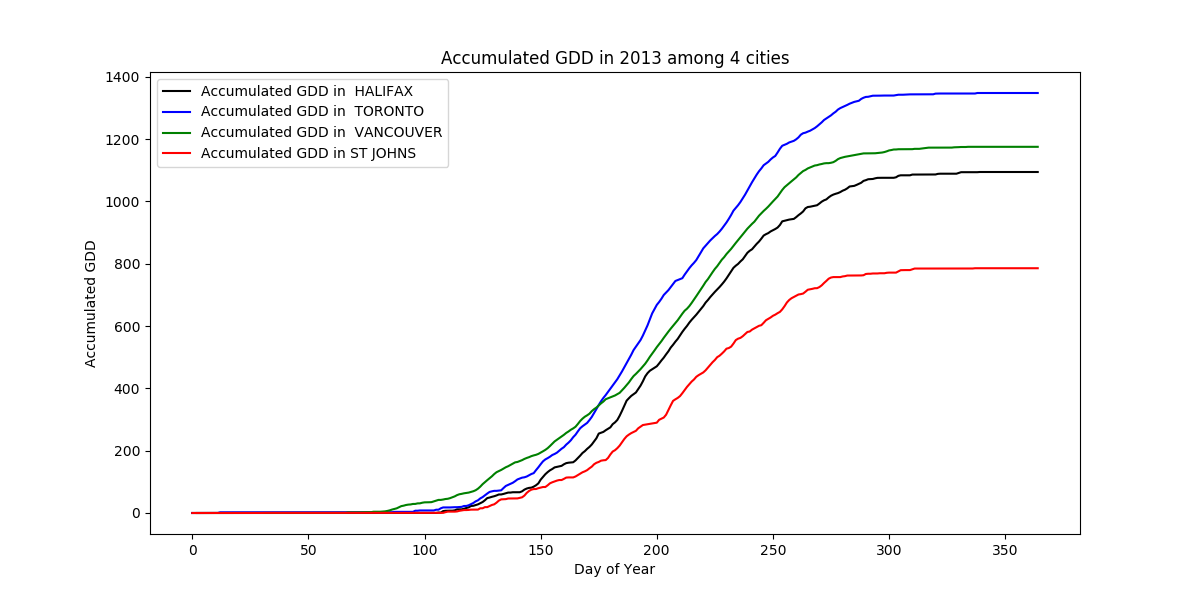
\includegraphics[width=5.25in]{Plot/accGDD_2013.png}



\caption{Accumulated GDD in 2013}
\label{5}
\end{figure}


\subsection{Year 2014}

In year 2013, the accumulated GDD of Vancouver takes the lead, followed by Toronto, Halifax and St.John's.
\begin{figure}[H]
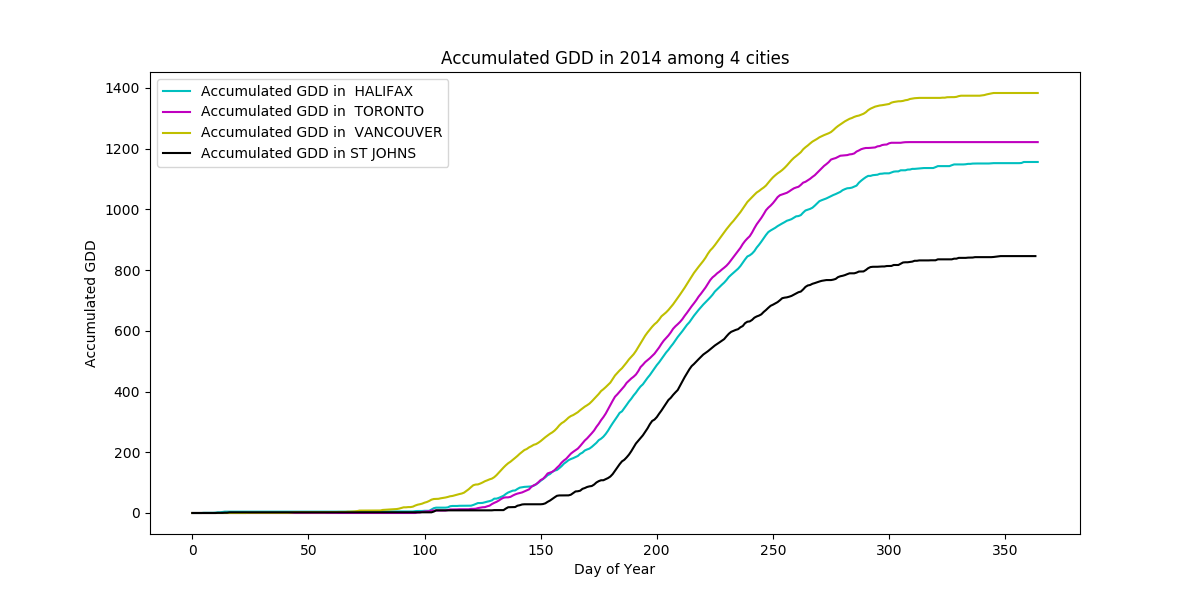
\includegraphics[width=5.25in]{Plot/accGDD_2014.png}



\caption{Accumulated GDD in 2014}
\label{5.2}
\end{figure}

\subsection{Year 2015}
In year 2013, the accumulated GDD of Vancouver takes the lead, followed by Toronto, Halifax and St.John's.
\begin{figure}[H]
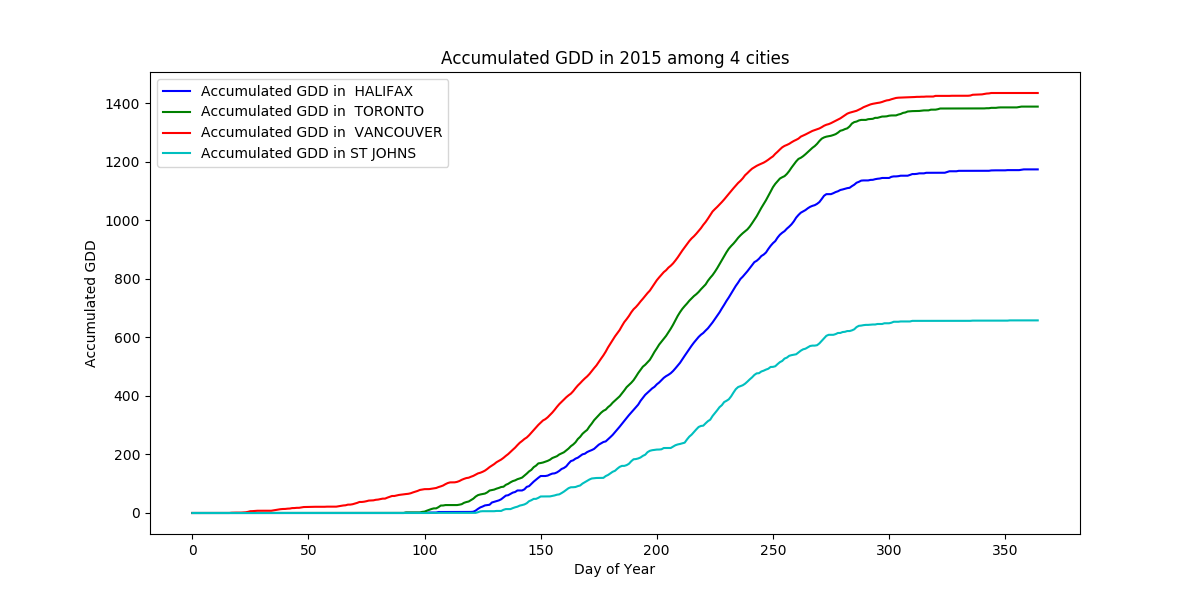
\includegraphics[width=5.25in]{Plot/accGDD_2015.png}



\caption{Accumulated GDD in 2015}
\label{5.3}
\end{figure}

\subsection{Year 2016}
In year 2013, the accumulated GDD of Toronto takes the lead, followed by Vancouver, Halifax and St.John's.
\begin{figure}[H]
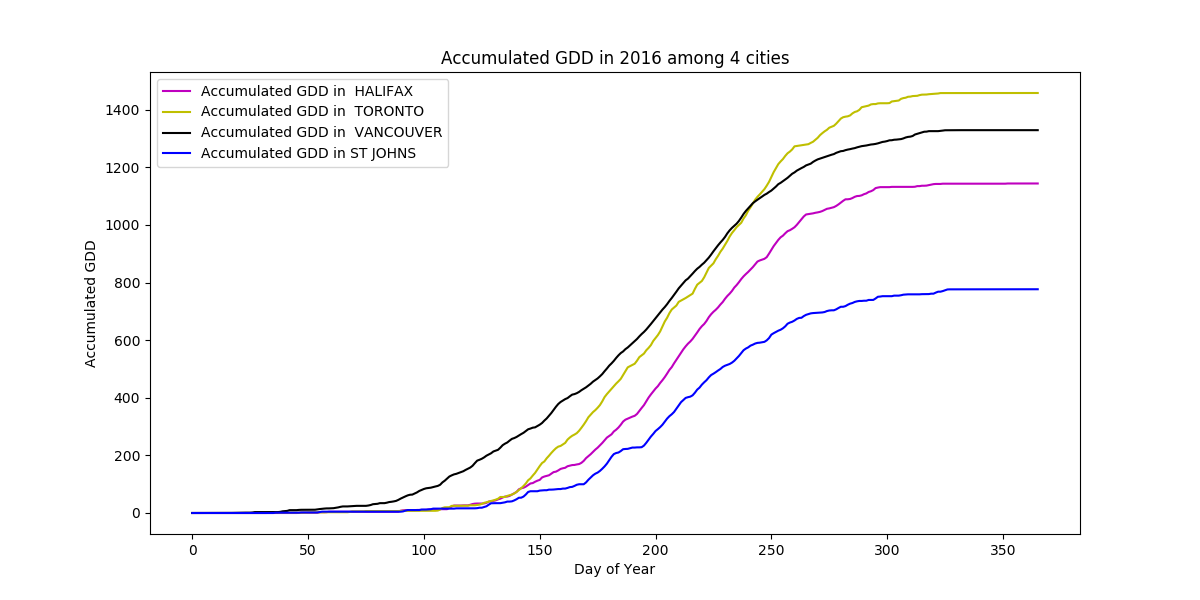
\includegraphics[width=5.25in]{Plot/accGDD_2016.png}



\caption{Accumulated GDD in 2016}
\label{5.4}
\end{figure}

In conclusion, between year 2013 and 2016, Toronto or Vancouver has the highest value of accumulated GDD, the accumulated GDD value of Halifax stays in the middle, St.John's has the lowest accumulated GDD. 



\subsection{ \bf Year to Year Accumulated GDD }
\subsection{St.John's}

From figure (\ref{5.1}), in year 2014, St.John's has the highest accumulated GDD among year 2013 to 2016. Moreover, its value is around 850. In year 2015, the value of accumulated GDD for St.John's is around 600, it is the lowest value of accumulated GDD among year 2013 to 2016. 

The difference of accumulated GDD between highest value to lowest value is around 250 for St.John's among year 2013 to 2016.

\begin{center}
\begin{figure}[H]
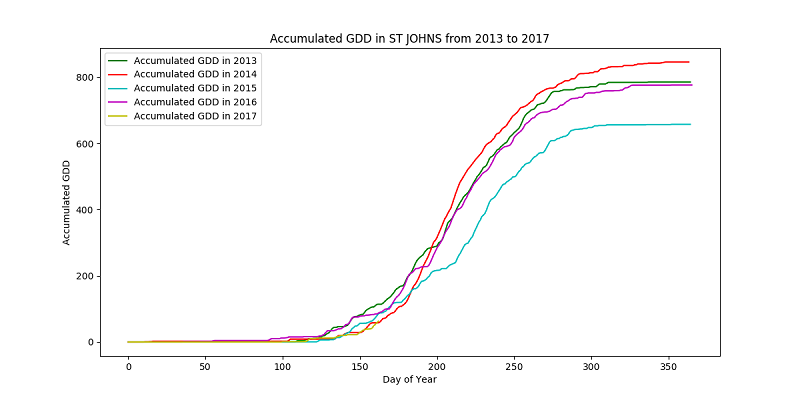
\includegraphics[width=5.25in]{Plot/yearst.png}




\caption{Accumulated GDD from 2013 to 2017 for St.John's.}
\label{5.1}
\end{figure}
\end{center}


\subsection{Halifax}

From figure (\ref{5.2}), in year 2015, Halifax has the highest accumulated GDD among year 2013 to 2016, its value is around 1100. In year 2013, the value of accumulated GDD for Halifax is around 1000, it is the lowest value of accumulated GDD among year 2013 to 2016. 

The difference of accumulated GDD between highest value to lowest value is around 100 for Halifax among year 2013 to 2016.

Compared to St.John's, the relative difference of accumulated GDD among year 2013 to 2016 is not as big as St.John's.
\begin{center}
\begin{figure}[H]
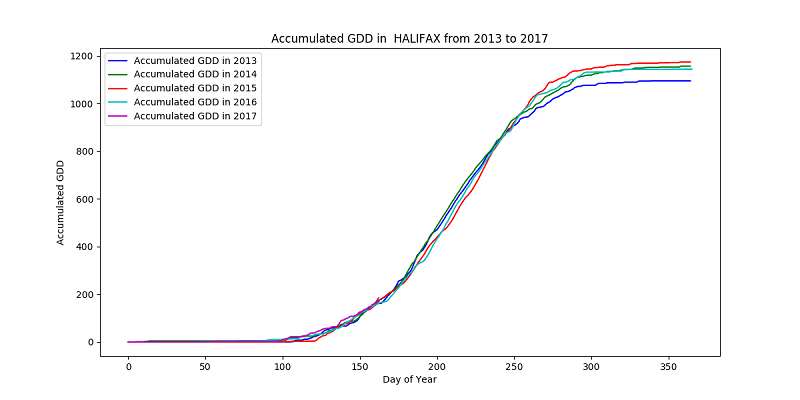
\includegraphics[width=5.25in]{Plot/yearha.png}
\caption{Accumulated GDD from 2013 to 2017 for Halifax.}
\label{5.2}
\end{figure}
\end{center}


\subsection{Toronto}

From figure (\ref{5.3}), in year 2016, Toronto has the highest accumulated GDD among year 2013 to 2016, its value is around 1500. In year 2014, the value of accumulated GDD for Halifax is around 1100, it is the lowest value of accumulated GDD among year 2013 to 2016. 

The difference of accumulated GDD between highest value to lowest value is around 400 for Toronto among year 2013 to 2016.

\begin{center}
\begin{figure}[H]
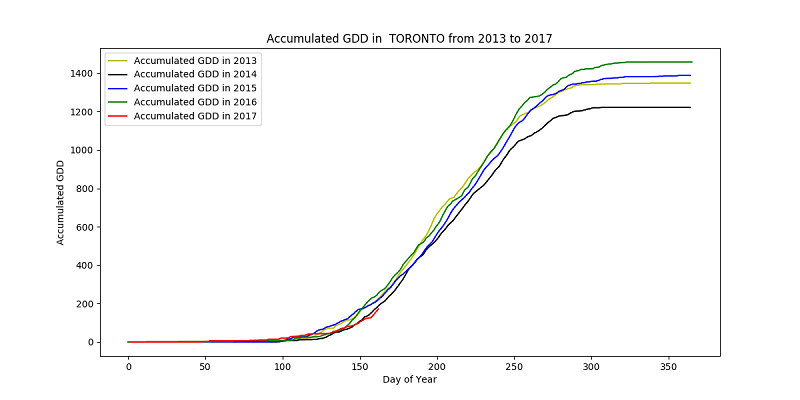
\includegraphics[width=5.25in]{Plot/yearto.png}
\caption{Accumulated GDD from 2013 to 2017 for Toronto.}
\label{5.3}
\end{figure}
\end{center}


\subsection{Vancouver}


From figure (\ref{5.4}), in year 2015, Vancouver has the highest acumulated GDD among year 2013 to 2016, its value is around 1400. In year 2013, the value of accumulated GDD for Halifax is around 1100, it is the lowest value of accumulated GDD among year 2013 to 2016. 

The difference of accumulated GDD between highest value to lowest value is around 300 for Vancouver among year 2013 to 2016.
\begin{center}
\begin{figure}[H]
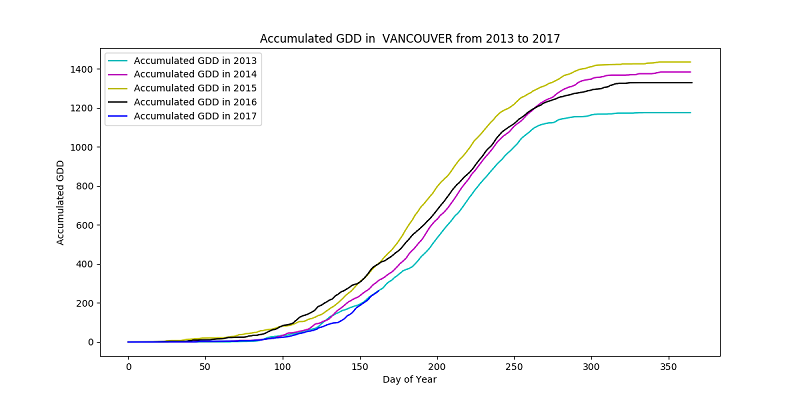
\includegraphics[width=5.25in]{Plot/yearvan.png}




\caption{Accumulated GDD from 2013 to 2017 for Vancouver.}
\label{5.4}
\end{figure}
\end{center}

In conclusion, the biggest difference of accumulated GDD among year 2013 to 2016 belongs to Toronto which has the value 400. The smallest difference of accumulated GDD among year 2013 to 2016 belongs to Halifax which has the value 100.

\subsection{Accumulated GDD Plot with Different Base Temperature}

\begin{center}
\begin{figure}[H]
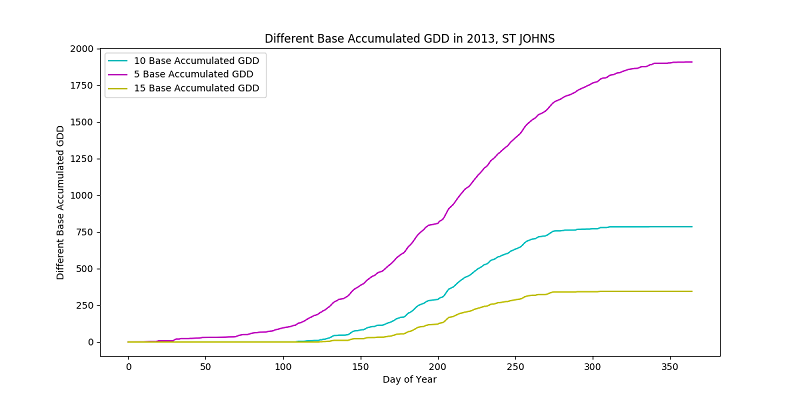
\includegraphics[width=5.25in]{Plot/differentT_baseforStJohns.png}
\caption{Accumulated GDD with different base temperature for St.John's in 2013.}
\label{5.5}
\end{figure}
\end{center}




\begin{center}
\begin{figure}[H]
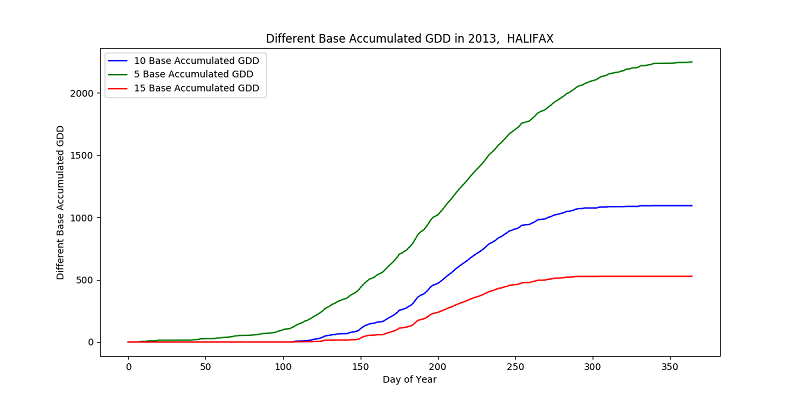
\includegraphics[width=5.25in]{Plot/differentT_baseforHalifax.png}

\caption{Accumulated GDD with different base temperature for Halifax in 2013.}
\label{5.6}
\end{figure}
\end{center}




\begin{center}
\begin{figure}[H]
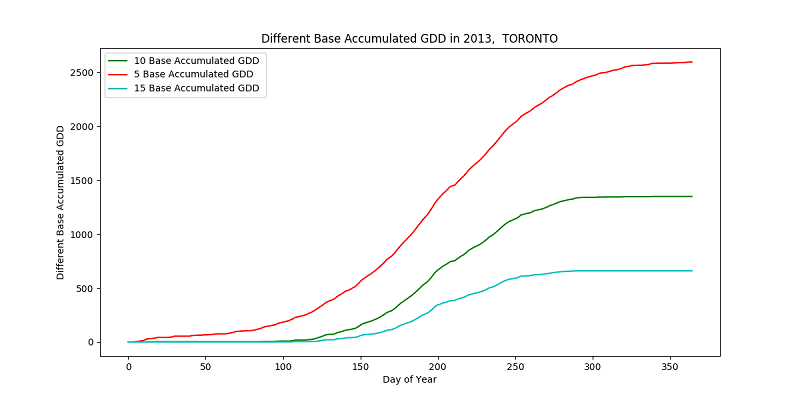
\includegraphics[width=5.25in]{Plot/differentT_baseforToronto.png}
\caption{Accumulated GDD with different base temperature for Toronto in 2013.}
\label{5.7}
\end{figure}
\end{center}




\begin{center}
\begin{figure}[H]
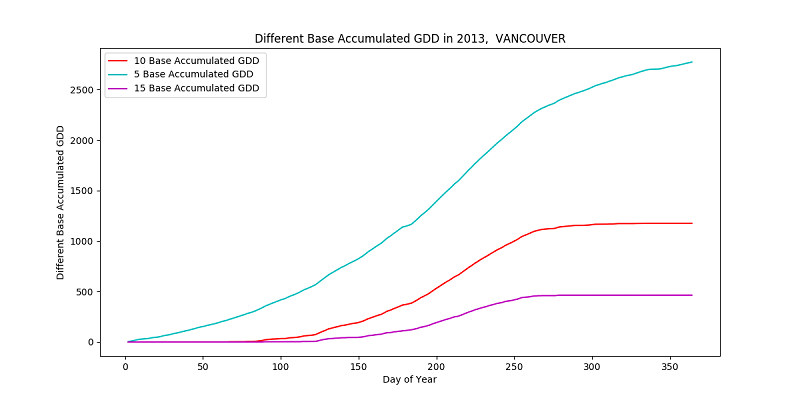
\includegraphics[width=5.25in]{Plot/differentT_baseforVancouver.png}
\caption{Accumulated GDD with different base temperature for Vancouver in 2013.}
\label{5.8}
\end{figure}
\end{center}
\section{ \bf Discussion}
From our plots we can see that from year 2013 to year 2016, the accumulated GDDs for our selected cities are not increased year by year. Moreover, the difference of accumulated GDD for Halifax is not as big as Toronto, one reason may be that Toronto is a city in the middle of Canada, it is away from the ocean, therefore, the daily temperature may change differently from year to year. However, Halifax is near ocean, therefore, the daily temperature may remain close year to year. 

For city St.John's, the accumulated GDD is relatively low compare to other selected cities. Although the difference between the highest accumulated GDD value and lowest accumulated GDD value among year 2013 to 2016 is only 250, it is still relatively a big change since the highest value of accumulated GDD is around 800. Therefore, the daily temperature of St.John's also has a relatively big change.


\section{Conclusion}
From our project, we can predict that those flowers can bloom in St.John's, it is also can blooming in Halifax, Toronto and Vancouver. However, for some agriculture plants such as wheat (need 1550-1680 GDD to maturity) can not grow well in St.John's and Halifax. Barley (need 1290-1540 GDD to maturity) can grow in Halifax but not in St.John's. Moreover, for some insect such as oats (1500-1750 GDD to maturity) can not live in Halifax and St.John's.




\section{References}

\begin{enumerate}
\item \href{url}{$https://en.wikipedia.org/wiki/Growing_degree-day$}
\item \href{url}{$http://climate.weather.gc.ca/$}
\end{enumerate}


\end{document}
